\chapter{Overzicht bestaande representaties}

Om te kijken wat er in de praktijk gebruikt wordt op het gebied van bewegwijzering in multifunctionele gebouwen zijn we gaan kijken in de RAI Amsterdam, AHOY Rotterdam en in het VU Academisch Ziekenhuis Amsterdam.

In multifunctionele gebouwen is de bewegwijzering onder te verdelen in twee soorten: permanente bewegwijzering en evenement-specifieke bewegwijzering. We bekeken van beide soorten bestaande representaties.


\section{RAI Amsterdam} \label{sectie:overzicht_rai}

In het RAI complex hebben de hallen en zalen respectievelijk nummers en letters. Ze hebben ook namen, maar deze worden in de bewegwijzering vrijwel niet gebruikt.

\begin{itemize}

\item \emph{Permanente bewegwijzering}

\begin{itemize}
\item In de hallen hangen vanen met halnummers aan het plafond. In iedere hal is zo gemakkelijk te zien waar je je bevindt.
\item Aan de muren hangen grote plattegronden die situatie-gericht zijn (zie figuur~\ref{figuur:rai_plattegrond}). Deze hangen door heel het complex verspreid.

\begin{figure}
\begin{center}
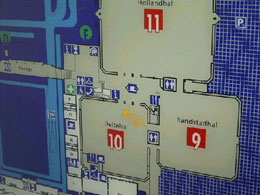
\includegraphics{images/rai_plattegrond.jpg}
\end{center}
\caption{Voorbeeld van een plattegrond (RAI)}
\label{figuur:rai_plattegrond}
\end{figure}

\item In vrijwel alle ruimtes vinden we blauwe bordjes voor faciliteiten als garderobe, WC, brandblussers en naar andere hallen en zalen. Deze bordjes zijn voorzien van pijltjes om de richting aan te geven.
\item In enkele gangen hangen electronisch programmeerbare borden. Deze bieden slechts een minieme ondersteuning en zijn erg beperkt programmeerbaar.
\end{itemize}

\item \emph{Evenement-specifieke bewegwijzering}

\begin{itemize}
\item Buiten staan grote blauwe zuilen waarin voor ieder evenement borden geschoven kunnen worden (zie figuur~\ref{figuur:rai_zuil}).

\begin{figure}
\begin{center}
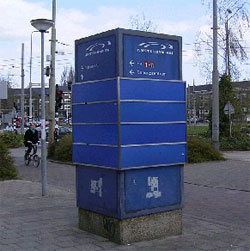
\includegraphics{images/rai_zuil.jpg}
\end{center}
\caption{Voorbeeld van een zuil (RAI)}
\label{figuur:rai_zuil}
\end{figure}

\item Bewegwijzering naar parkeerplaatsen verschilt ook per evenement, vooral afhankelijk van de drukte.
\end{itemize}

Overige evenement-specifieke bewegwijzering wordt niet door de RAI geregeld, maar door de organisatie van het betreffende evenement.

\item \emph{Niet-standaard bewegwijzering}

In het geval van onvoorziene omstandigheden, zoals een defecte lift, worden er door de RAI kleine witte zuilen geplaatst waarop simpele boodschppen op A4 formaat gehangen kunnen worden.

\end{itemize}


\section{AHOY Rotterdam} \label{sectie:overzicht_ahoy}

In het AHOY complex hebben de verschillende zalen en hallen ook nummers en namen. AHOY gebruikt voor de bewegwijzering echter bij voorkeur geen van deze twee. Op de borden in AHOY staan alleen de namen van de evenementen vermeld. De filosofie hier achter is dat de bezoeker niets heeft aan een zaalnummer of -naam, maar wil weten waar hij zijn of haar evenement kan vinden.

In AHOY was weinig echt permanente bewegwijzering aanwezig, behalve bordjes bij faciliteiten zoals WC, lift, garderobe, etcetera. Permanente bordjes om een richting of route te wijzen waren er vrijwel niet.

\begin{itemize}

\item \emph{Permanente bewegwijzering}

\begin{itemize}
\item Bij de ingangen van hallen en zalen hangen borden met nummer en/of naam.
\item Bij faciliteiten als WC, lift en garderobe hangen bordjes met iconen.
\item In de ruimte tussen de hallen hangen bewegwijzeringsbordjes met iconen (zie figuur~\ref{figuur:ahoy_borden}).

\begin{figure}
\begin{center}
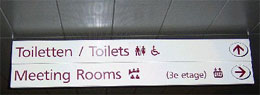
\includegraphics{images/ahoy_borden.jpg}
\end{center}
\caption{Voorbeeld van bewegwijzering (AHOY)}
\label{figuur:ahoy_borden}
\end{figure}

\end{itemize}

\item \emph{Evement-specifieke bewegwijzering}

\begin{itemize}
\item In de gangen van het complex staan verplaatsbare zuilen waarin bewegwijzerings-bordjes gehangen kunnen worden (zie figuur~\ref{figuur:ahoy_zuil}). Deze bordjes worden voor ieder evenement door de huisdrukker van AHOY gemaakt.

\begin{figure}
\begin{center}
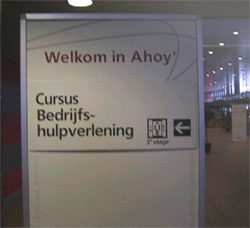
\includegraphics{images/ahoy_zuil.jpg}
\end{center}
\caption{Voorbeeld van een zuil (AHOY)}
\label{figuur:ahoy_zuil}
\end{figure}

\item In de tweede helft van 2003 hoopt AHOY electronische borden te introduceren. De bedoeling is dat deze op vaste plaatsen komen te hangen en de verplaatsbare zuilen zullen vervangen.
\end{itemize}

\end{itemize}


\section{VU Academische Ziekenhuis Amsterdam}

Hoewel in het VU Academisch Ziekenhuis eigenlijk geen echt multifunctionele ruimten zijn in dezelfde zin als dat het geval is in een beurscomplex, is de complexiteit van de bewegwijzering zeker te vergelijken. Deze bestond tijdens ons bezoek aan het ziekenhuis uit een permanent systeem van borden (dit was vrij recent ge\"\i nstalleerd) en een ge\"\i mproviseerd systeem van gele A4-tjes. Op deze gele A4-tjes werden ook tijdelijke omleidingen aangegeven.

Verschillende gebouwen worden in het ziekenhuis met letters (A t/m E), verdiepingen met nummers en kamers met nummers aangegeven.

We maken voor het VU Academisch Ziekenhuis het onderscheid tussen permanente en tijdelijke bewegwijzering, evenement-specifieke bewegwijzering is in het ziekenhuis uiteraard niet van toepassing.

\begin{itemize}

\item \emph{Permanente bewegwijzering}

\begin{itemize}
\item In veel gangen en lift-hallen hangen zilverkleurige borden met daarop gebouwletter, verdieping en reeks kamernummers (zie figuur~\ref{figuur:vu_nieuw}).

\begin{figure}
\begin{center}
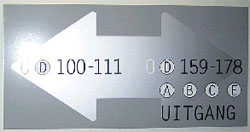
\includegraphics{images/vu_nieuw.jpg}
\end{center}
\caption{Voorbeeld van bewegwijzering (VU Ziekenhuis)}
\label{figuur:vu_nieuw}
\end{figure}

\item Door heel het complex hangen bordjes bij faciliteiten als WC en garderobe.
\item Bij ingangen van kamers zijn bordjes geplaatst met het kamernummer, omschrijving en eventueel namen van personen die in de kamer werken.
\item In sommige gangen zijn nog bordjes te vinden van het oude bewegwijzeringssysteem, waarop de gebouwen met Noord, Oost, Zuid en West aangeduid worden, in plaats van met letters (zie figuur~\ref{figuur:vu_oud}).

\begin{figure}
\begin{center}
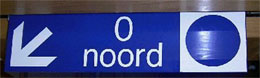
\includegraphics{images/vu_oud.jpg}
\end{center}
\caption{Voorbeeld van oude bewegwijzering (VU Ziekenhuis)}
\label{figuur:vu_oud}
\end{figure}

\end{itemize}

\item \emph{Tijdelijke bewegwijzering}

\begin{itemize}
\item Op gele blaadjes zijn gebouwletter, verdieping en reeks kamernummers met richting aangegeven.
\item Op de begane grond zijn gele blaadjes aanwezig met daarop uitgelegd hoe de inhoud van de gele blaadjes te interpreteren (zie figuur~\ref{figuur:vu_uitleg}).

\begin{figure}
\begin{center}
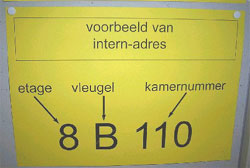
\includegraphics{images/vu_uitleg.jpg}
\end{center}
\caption{Uitleg van intern-adres (VU Ziekenhuis)}
\label{figuur:vu_uitleg}
\end{figure}

\item Een enkele keer worden witte A4-tjes met geschreven tekst gebruikt om een richting aan te geven.
\end{itemize}

\end{itemize}
